\documentclass{article}
\usepackage{graphicx}
\usepackage[utf8]{inputenc}
\usepackage[T1]{fontenc}
\usepackage{pgfplots}
\usepackage{pgfplotstable} 
\usepackage{titlesec}
\usepackage{lipsum}
\usepackage{authblk}
\usepackage{algorithm}
\usepackage{amsmath}
\usepackage[noend]{algpseudocode}
\usepackage {tikz}
\usetikzlibrary {positioning}

\titleformat{\chapter}[display]{\normalfont\bfseries}{}{0pt}{\Large}

\begin{document}

\title{Projeto e Análise de Algoritmos: Trabalho Prático 1}
\author{João Mateus de Freitas Veneroso}
\affil{Departamento de Ciência da Computação da Universidade Federal de Minas Gerais}

\maketitle

\section{Introdução}

Este relatório descreve a implementação do trabalho prático 2 da disciplina Projeto e Análise de Algoritmos. 
O trabalho consistiu em resolver um problema de compartilhamento de viagens por meio de três paradigmas diferentes:
força bruta, programação dinâmica e algoritmos gulosos.

\section{Força Bruta}

O algoritmo de força bruta descrito abaixo é o mesmo implementado no Trabalho Prático 1.

O algoritmo \ref{alg:alg_1} implementa uma solução de força bruta para o problema de compartilhamento de viagens. 
Primeiro inicializa-se o benefício máximo $ b^* $ com um valor negativo, dessa
forma qualquer configuração válida vai proporcionar um benefício maior. A partir daí, no loop das linhas 5-10, para cada configuração
válida, calcula-se o benefício total e atualiza-se o valor de $ b^* $ se este benefício for maior do que qualquer um encontrado até então.
Além disso, a variável $ G_p^* $ guarda a configuração que proporcionou o maior benefício. Ao final do algoritmo, $ b^* $ guarda o valor 
do benefício máximo para o grafo $ G $ e $ G_p^* $ guarda a configuração que proporcionou este benefício. 

A complexidade deste algoritmo depende do número de configurações $ G_p $ diferentes e do custo da função $ ConstraintsAreValid $. O número de 
configurações $ G_p $ diferentes é $ 2^m $ para $ m $ igual ao número de arestas no grafo $ G $. Pois, cada aresta pode estar presente ou
não em $ G_p $ e nós queremos as combinações possíveis para todas as arestas m. O custo da função $ ConstraintsAreValid $ depende do número de 
arestas, pois, para cada aresta $ (u,v) $, temos de verificar se ela é a única aresta que sai do vértice $ u $, se o vértice $ v $ é um motorista
e se $ v $ possui espaço para acomodar todos os passageiros de $ u $. Como todas estas operações tem custo constante, a função $ ConstraintsAreValid $ 
tem custo $ O(m) $. Por último, a linha 7 calcula a soma dos pesos de todas as arestas também com custo $ O(m) $. Logo, 
a complexidade total do algoritmo é $ 2m2^m $ e o algoritmo é $ O(m2^m) $.

\begin{algorithm}
\caption{MaximizeBenefit}\label{euclid}
\begin{algorithmic}[1]
\Procedure{MaximizeBenefit}{G = (V,A)}

\State $ b^* \gets -1 $
\State $ G_p^* \gets \emptyset $
\item \ForAll{\textit{$ G_p = (V, A_p) : A_p \subseteq G.A $}}

\If {\textit{ConstraintsAreValid($G_p$)}}
  \State $ \textit{b} \gets \sum_{(v_i, v_j) \in A_p} B(v_i, v_j) $
  \If {$ b > b^* $}
    \State $ b^* \gets b $
    \State $ G_p^* \gets G_p $
  \EndIf
\EndIf
\EndFor
\EndProcedure
\end{algorithmic}
\label{alg:alg_1}
\end{algorithm}

Uma melhora ainda pode ser alcançada se deixarmos de testar parte das configurações inválidas de $ G $. Sabemos que 
um passageiro só pode pegar carona em uma rota, portanto, qualquer combinação $ G_p $ onde existirem arestas $ (u, v_i), (u, v_j) : i \neq j $
é inválida. Dessa forma, basta manter uma única aresta ativa por vez na lista de adjacência de cada vértice. Por exemplo, na figura \ref{fig:graph} apenas 
duas combinações precisam ser testadas: $ G_0(V,A_0) : A_0 = \{(X,Y)\} $ e $ G_1(V,A_1) : A_1 = \{(X,Z)\} $.

Além disso, é necessário lembrar que um vértice pode representar um motorista sem passageiros ou um passageiro que não vai pegar carona com ninguém, 
portanto, o número total de combinações 
se torna $ \sum_{v \in V} G \rightarrow Adj(v) + 2 $ e, no pior caso (um grafo completo), o número de combinações se torna $ O(n^n) $ 
onde n é o número de vértices no grafo $ G $. Feitas estas considerações, a complexidade assintótica do algoritmo é $ O(mn^n) $.
O algoritmo implementado em Python para este trabalho utiliza este método.

A complexidade de espaço do algoritmo original e da versão aprimorada é $ O(n + m) $, pois o grafo é armazenado na forma de listas de adjacência.

\section{Programação Dinâmica}

No problema do compartilhamento de viagens modelado em grafos, os vértices do grafo representam viagens e as arestas do grafo representam 
compartilhamentos. Cada vértice pode representar viagens com passageiros exclusivos, motoristas exclusivos 
ou passageiros-motoristas. Em qualquer solução válida os passageiros-motoristas tem de decidir se vão
atuar como passageiros ou motoristas devido às restrições do problema. Dessa forma, sendo k o número de passageiros-motoristas, 
ao variar quais deles atuam como passageiros e quais atuam como motoristas, existem $ 2^k $ combinações possíveis que dão origem a problemas distintos. 
Cada um destes problemas pode ser pensado como um grafo bipartido G(V,A) onde os vértices de passageiros pertencem a um subconjunto de V e os vértices 
de motoristas pertencem a um outro subconjunto de V, sendo que todas as arestas conectam um vértice passageiro a um vértice motorista e os dois subconjuntos
são disjuntos.

\begin{figure}
  \center
  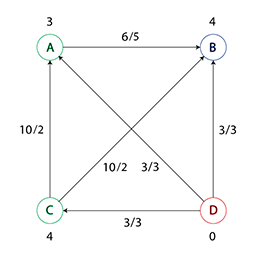
\includegraphics[width=128px]{graph.png}
  \caption{Exemplo do problema de compartilhamento de viagens modelado em forma de grafo}
  \label{fig:graph}
\end{figure}

\begin{figure}
  \center
  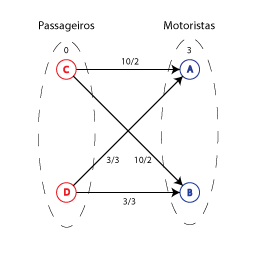
\includegraphics[width=164px]{bipartite_graph.png}
  \caption{Grafo bipartido após definição dos passageiros e motoristas no grafo da figura \ref{fig:graph}}
  \label{fig:bipartite_graph}
\end{figure}

A figura \ref{fig:graph} mostra um exemplo do probema de compartilhamento de viagens modelado na forma de um grafo, onde vértices
vermelhos representam grupos de passageiros, vértices azuis representam motoristas e vértices verdes representam passageiros-motoristas. Os números
próximos aos vértices representam a capacidade do veículo e os números próximos às arestas $ (v_i, v_j) $ representam o 
benefício do compartilhamento $ B(v_i, v_j) $ e o número de passageiros na viagem $ Q(v_i, v_j) $ separados por uma barra.
Perceba que os vértices A e C são passageiros-motoristas e os demais vértices são passageiros ou motoristas exclusivos. Ao selecionar 
o vértice A como motorista e o vértice C como passageiro, podemos modelar o problema com o grafo bipartido da figura \ref{fig:bipartite_graph}.
Para cada uma das combinações de passageiros e motoristas podemos construir um grafo bipartido similar. Nesta forma, o problema passa a se parecer
bastante com o \textit{0-1 Multiple Knapsack Problem}, com a diferença que alguns items podem estar restritos à sacolas específicas. 
No caso, as sacolas representam os carros e os itens representam os grupos de passageiros.
Além disso, é possível mapear o \textit{0-1 Multiple Knapsack Problem} no problema de compartilhamento de viagens se considerarmos 
o caso em que todos os passageiros podem pegar carona em todos os veículos. Logo, o problema do compartilhamento de viagens é NP-difícil.

Dado um grafo $ G(V,A)$, cada motorista $ v_j $ dá origem a um \textit{0-1 Knapsack Problem}. Pois, cada aresta $ (v_i, v_j) \in G.A $
representa uma possbilidade do grupo de passageiros $ v_i $ seguir viagem com $ v_j $. E, para maximizar o benefício dos
compartilhamentos do motorista $ B_{max}(G, v_j) $ é preciso escolher o conjunto de arestas $ (v_i, v_j) $ que confira o maior benefício
sem exceder a capacidade do carro, que é basicamente a definição do \textit{0-1 Knapsack Problem}. No entanto, a forma como 
um motorista maximiza o benefício dos seus compartilhamentos influencia como os outros motoristas podem
maximizar os seus compartilhamentos. Logo, assumindo que o motorista $ v_j $ está levando o grupo de passageiros $ X $, o próximo
motorista deverá maximizar seu benefício com base no grafo $ G'(V - X - v_j, A') $, sendo que $ A' $ é o conjunto de arestas original 
$ A $ sem as arestas que contém $ v_j $ ou qualquer um dos passageiros levados. No caso de motoristas que podem ser passageiros,
também existe a possibilidade do motorista $ v_j $ não levar passageiro nenhum. Nesse caso, as arestas incidentes em $ v_j $
serão apagadas do grafo $ G $, mas as arestas que saem de $ v_j $ serão mantidas e, o vértice $ v_j $ também será mantido.

Se o motorista $ v_j $ decide levar um passageiro $ v_i $, os demais motoristas vão maximizar seus benefícios sem considerar o 
passageiro $ v_i $ no grafo. Por conta disso, o benefício encontrado não será necessariamente máximo. Por exemplo, tome o caso em que
$ v_j $ pode levar um dos grupos de passageiros $ \{ p_1 = 12/2, p_2 = 20/1, p3 = 1/1 \} $ onde o primeiro valor associado a cada grupo representa o seu benefício
e o segundo valor o número de pessoas naquele grupo (note que a barra não representa divisão nesse caso).
Assumindo que $ v_j.capacidade = 2 $, $ v_j $ maximiza o benefício dos seus compartilhamentos se escolher os passageiros $ \{ p_2, p_3 \} $ auferindo um
benefício total de $ 21 $. Agora assuma que existe um outro motorista $ v_{j+1} $ que pode compartilhar viagem apenas com $ p_2 $. Nesse caso,
o motorista $ v_{j+1} $ ficará impedido de compartilhar essa viagem. No entanto, o benefício máximo dos compartilhamentos seria claramente 
maior se $ v_j $ tivesse escolhido levar $ p_1 $ ao invés de $ \{ p_2, p_3 \} $. 

Por conta da incapacidade de prever localmente qual é o benefício total máximo do plano de compartilhamento, é necessário testar 
cada uma das combinações de $ k $ passageiros para o motorista $ v_j $ e escolher aquela que provê o benefício total máximo.
Isto dá um total de $ 2^k $ combinações, onde, para cada combinação de passageiros, constrói-se um grafo $ G' $ sem aqueles passageiros
e sem o motorista ou apenas sem as arestas dos passageiros se o motorista não for levar ninguém, como explicado anteriormente. 
Então, calculamos o benefício máximo para o subgrafo $ G' $ e assim por diante. Sendo que cada combinação de passageiros em 
cada motorista pode ter seu benefício máximo calculado pela resolução do \textit{0-1 Knapsack Problem}.

Finalmente, podemos construir a seguinte equação de recorrência:

\begin{equation}
  B_{max}(G, D_{j}) = 
  \begin{cases}
    0, & \textit{se $ G = \emptyset $}.\\
    \max_{P_k \subseteq D_j.P} B_{max}(G', D_{j+1}) + B(P_k), & \textit{caso contrário}.\\
  \end{cases}
\end{equation}

onde $ P_k $ são todos as combinações de passageiros do motorista $ D_j $, onde $ P_k \subseteq D_j.passageiros \subseteq G.A $.
$ G' $ depende da escolha dos passageiros como explicado nos parágrafos anteriores e $ B(P_k) $ é o somatório dos benefícios
dos passageiros em $ P_k $. A ordem de escolha dos motoristas $ D_j $ não é importante uma vez que todas as possíveis combinações de
passageiros acabam sendo testadas de uma forma ou de outra. No entanto, esta ordem será importante quando tratarmos da solução gulosa para o problema.

Perceba que para calcularmos o benefício máximo de $ G $ é necessário resolver maximizar os benefícios nos subproblemas $ G' $. 
Ou seja, o problema tem subestrutura ótima. A prova deste postulado é que, se obtemos o benefício máximo em $ G $ com base
em um $ B(G') $ cujo benefício não é máximo, então, podemos simplesmente substituir $ B(G') $ por $ B_{max}(G') $ e obter um benefício
maior, contradizendo o fato de $ G $ ser máximo inicialmente. Portanto, $ B(G') $ tem de ser máximo.

A implementação ingênua desta equação de recorrência acaba calculando várias vezes o mesmo problema, pois, um subgrafo $ G' $ pode ocorrer
diversas vezes na árvore de recursão, mas o seu benefício máximo $ B_max(G') $ é sempre o mesmo. Portanto, podemos ganhar eficiência ao
salvar os resultados dos cálculos anteriores do \textit{0-1 Knapsack Problem}. Além disso, podemos utilizar uma abordagem de programação
dinâmica para resolver o próprio \textit{0-1 Knapsack Problem}.

O \textit{0-1 Knapsack Problem} pode ser resolvido de forma simples gerando uma tabela onde as linhas representam os passageiros
$ \{ p_1, p_2, ..., p_n\} \in D_j.P $ e as colunas representam a capacidade de $ D_j $ de 1 até $ D_j.capacidade $. Então, calculamos
para cada linha, o benefício máximo com cada uma das colunas de capacidade. Na próxima linha, verificamos se podemos incluir o próximo passageiro 
para cada uma das capacidades e, se isso não for possível, repetimos o valor da célula de cima. Se for possível incluir o passageiro, então
verificamos o valor da linha de cima com a capacidade da coluna atual menos o número de passageiros adicionados. Devido a uma limitação
de espaço este algoritmo não será explicado em mais detalhes. No entanto, o código implementa ele conforme os passos aqui descritos.

No caso do cálculo do benefício máximo, podemos seguir uma abordagem \textit{Bottom Up}. Digamos que $ D = {D_1, D_2, ..., D_n} $ é
a lista dos motoristas no grafo G.





\end{document}
